\documentclass[11pt]{article}

\usepackage[margin=1in]{geometry}
\usepackage{amsmath, amssymb, amsthm}
\usepackage{mathtools}
\usepackage{booktabs}
\usepackage{tabularx}
\usepackage{graphicx}
\graphicspath{{figures/}{../figures/}}
\usepackage[hidelinks]{hyperref}
\usepackage[authoryear,round]{natbib}
\bibpunct{(}{)}{,}{a}{}{,}

\newcommand{\R}{\mathbb{R}}
\newcommand{\E}{\mathbb{E}}
\newcommand{\F}{\mathcal{F}}
\newcommand{\pluspart}[1]{\left[#1\right]_+}
\newcommand{\minuspart}[1]{\left[#1\right]_-}

\theoremstyle{plain}
\newtheorem{theorem}{Theorem}
\newtheorem{lemma}{Lemma}
\newtheorem{proposition}{Proposition}
\theoremstyle{definition}
\newtheorem{definition}{Definition}
\newtheorem{assumption}{Assumption}
\theoremstyle{remark}
\newtheorem{remark}{Remark}

\title{Optimal Trading Filters: a Wiener--Hopf Approach}
\author{Matteo Smerlak\thanks{Capital Fund Management, 23 rue de l'Universit\'e, 75007 Paris, France. \texttt{matteo.smerlak@cfm.com}}}
\date{}

\begin{document}
\maketitle

\begin{abstract}
We consider the optimal trading problem: given a return-predicting signal, find the trading policy that maximizes expected gain net of temporary and transient impact costs, and possibly inventory risk. Existing treatments characterize the optimal policy implicitly, as the solution of an integral equation or an equivalent forward--backward system. We show that, away from horizon endpoints, the optimal trading filter can be computed in closed form using a Wiener--Hopf factorization of the friction operator. In the empirically motivated case of pure power-law transient impact, the optimal trading rate reduces to a fractional derivative of the signal of order $\nu = (1-\beta)/2$ with $\beta$ the impact decay exponent. The power-law policy generates no block trades and never reverses against the signal. The classical portfolio and execution rules --- the Markowitz position, the aim portfolio, the exponential-resilience filters, and the finite-horizon liquidation profiles --- are recovered as rational and scale-free special cases of the factorization.
\end{abstract}

% =====================================================================
\section{Introduction}\label{sec:intro}

\subsection{The gain--risk--cost problem}\label{sec:problem}

Optimal execution studies how to build or unwind a position when trading moves the price against the trader \citep{AlmgrenChriss2001,GatheralSchiedSlynko2012}. A return-predicting signal sharpens the problem: a forecast invites a position, but the trade that captures it pushes the price away, commits capital to risk, and takes time the forecast may not survive. The trader weighs the gain a signal promises against the cost of realizing it and the risk of holding it, acting on the information in hand and never on the signal's future.

Concretely, a trader observes a return signal $\mu_t$, the conditional expectation at time $t$ of the asset's instantaneous price drift, and chooses a position $x_t$ traded at the rate $u_t=\dot x_t$. Trading incurs friction in three ways. An inventory cost penalizes holding large positions. A temporary impact cost, quadratic in the rate, prices the demand for immediate liquidity. A transient impact cost carries the memory that each trade moves the price against later trades, decaying through a propagator kernel $g$ \citep{BouchaudGefenPottersWyart2004,Gatheral2010}. 

\citet{AlmgrenChriss2001} split the cost of trading in two: a temporary part, felt only by the trade that causes it, and a permanent part, linear in cumulative volume and left behind for every later trade. Minimizing the resulting mean--variance functional produced closed-form execution schedules. Empirical work then dissolved the sharp split: \citet{LilloFarmerMantegna2003} found impact to be a concave function of size, and \citet{BouchaudGefenPottersWyart2004} found it \emph{transient}, a trade displacing the price and the displacement relaxing, so that permanent and temporary costs are the slow and fast limits of one decaying response. This is the propagator picture, in which the price carries a weighted memory of past trades through a kernel $g$, and the shape of $g$ is the modeling choice.

Two shapes bracket that choice. Transaction data place $g$ near a \emph{power law}, $g(t)=t^{-\beta}$ with $\beta\in(0.2,0.6)$ \citep{BouchaudGefenPottersWyart2004,JusselinRosenbaum2020}, a scale-free decay with no characteristic time; \citet{Gatheral2010} showed a decay of about this form to be what no-dynamic-arbitrage allows, and \citet{JusselinRosenbaum2020} tied the exponent to rough volatility. At the other end, \citet{ObizhaevaWang2013} built impact from a limit order book of finite depth refilling at a fixed rate, an \emph{exponential} kernel $g(t)=e^{-\kappa t}$ with a single resilience time $1/\kappa$ whose fast and slow limits return the temporary and permanent costs of \citet{AlmgrenChriss2001}. The exponential kernel offers finite memory and closed forms; the power law has long memory and the empirical evidence.

The trader maximizes the expected gain of the position against the return, net of these costs,
\begin{equation}\label{eq:objective}
\max_{x\ \text{adapted}}\ \E\!\int x_t\mu_t\,dt
\;-\; \frac{\eta}{2}\,\E\!\int \dot x_t^2\,dt
\;-\; \frac{\gamma}{2}\,\E\!\iint g(|t-s|)\,\dot x_t \dot x_s\,dt\,ds
\;-\; \frac{\lambda}{2}\,\E\!\int x_t^2\,dt ,
\end{equation}
over positions adapted to the flow of information: $x_t$ may depend on the signal observed up to time $t$, not on its future. The integrals run over the whole line; Section~\ref{sec:boundary} poses the same problem on a finite window $[0,T]$ with a terminal inventory constraint. This paper gives exact solutions to \eqref{eq:objective} under both exponential and power-law impact kernels.


\subsection{The adaptedness constraint}\label{sec:adaptedness}


The objective \eqref{eq:objective} pairs a linear gain $\E\int x_t\mu_t\,dt$ against a positive quadratic cost $\tfrac12\E\langle x,Nx\rangle$ and thus evaluates the Legendre transform of the cost at $\mu$ under the adaptedness constraint. Specifically, the \emph{friction operator} $N$ collects the three costs referred to the position, $N=-\eta\,\partial_t^2-\gamma\,\partial_t^2(g\ast)+\lambda I$, with Fourier symbol
\begin{equation}\label{eq:symbol}
\hat n(\omega) \;=\; \eta\,\omega^2 \;+\; \gamma\,\hat g(\omega)\,\omega^2 \;+\; \lambda,
\qquad \hat g(\omega) = \int e^{i\omega t}g(|t|)\,dt \ge 0.
\end{equation}
Referred to the trading rate the friction is $Q=N\,(-\partial_t^2)^{-1}$, with symbol $\hat q=\hat n/\omega^2=\eta+\gamma\hat g+\lambda/\omega^2$, the form used for the scale-free kernel of Section~\ref{sec:fractional}. Unconstrained, the first-order condition of \eqref{eq:objective} is a single operator inversion, $x=N^{-1}\mu$.

With inventory cost alone ($\eta=\gamma=0$) the quadratic form is diagonal in time: the first-order condition at time $t$ involves $x_t$ and $\mu_t$ only, and the adapted optimum is the Markowitz rule $x_t=\mu_t/\lambda$ (Section~\ref{sec:recovery}). A temporary cost adds the local operator $-\eta\,\partial_t^2$, and the condition becomes an ordinary differential equation for the planned path, solved without factorization in Section~\ref{sec:recovery} (the aim portfolio). Transient impact removes this locality: its symbol $\gamma\hat g(\omega)\,\omega^2$ is not a polynomial, so $(Nx)(t)$ integrates the position over the past and the future, and adaptedness -- the requirement that $x_t$ be measurable with respect to $\F_t$ -- becomes binding. Varying \eqref{eq:objective} over adapted perturbations gives the first-order condition,
\begin{equation}\label{eq:foc}
\E_t\bigl[(Nx^\star)(t)\bigr] \;=\; \mu_t
\qquad\Longleftrightarrow\qquad
P_+\,N\,P_+\,x^\star = \mu,
\qquad (P_+X)_s = \E_s[X_s],
\end{equation}
with $P_+$ the optional projection onto adapted processes. Solving \eqref{eq:foc} requires inverting $P_+NP_+$, and the inverse of a projected operator is not the projection of the inverse, because $N$ is non-local.

\subsection{Causal factorization}\label{sec:thesis}

One way through is to factor $N$ along the filtration, into a causal factor and its anticausal adjoint: $N=N_-N_+$, with $N_+$ built from the past and invertible forward in time. Once $N$ splits this way the adapted inverse of $P_+NP_+$ can be assembled from the one-sided factors, and \eqref{eq:foc} is solved (Section~\ref{sec:interior}).

Factorizations of this kind go back to \citet{WienerHopf1931}, who introduced them for convolution equations on a half-line \citep{Krein1962,Noble1958}; there a support constraint couples the frequencies as the filtration couples them in \eqref{eq:foc}. Existence for a general positive operator came later --- \citet{GohbergKrein1970} for Volterra operators on an interval, \citet{Arveson1975} for positive operators on a nest of subspaces --- and the existence theorems do not by themselves produce the factor. The factor is explicit in the stationary case, where Fourier diagonalizes $N$ and the causal factor is the scalar Szeg\H{o} outer function, a frequency-domain route that also solves linear-quadratic dynamic optimization in economics \citep{Whiteman1985}; on a finite horizon translation invariance is lost, and the factor is explicit only for the special kernels of Section~\ref{sec:boundary}.

The factorization is also cheap to evaluate. Solving the first-order condition \eqref{eq:foc} numerically discretizes it to a dense triangular system whose size is the number of time steps $n$, at a cost of order $n^2$ paid afresh for each parameter set. The factorization returns the solution operator once and for all: on the whole line the optimal trade is a fixed convolution filter, applied in a single pass, and for a rational symbol it collapses to a handful of exponential moving averages that the trader updates in constant memory per step.

Section~\ref{sec:interior} solves the stationary problem in three steps --- factor the friction, predict the signal from its past, and combine the two --- through a projected-inverse identity (Lemma~\ref{lem:pi}) that assembles the adapted optimum for a general signal (Theorem~\ref{thm:general}) and, for stationary Gaussian signals, an explicit trading filter (Theorem~\ref{thm:filter}). The remaining sections draw out the consequences. Section~\ref{sec:fractional} collects the peculiarities of pure power-law impact: a fractional-derivative policy and a trade that never reverses against the signal. Section~\ref{sec:boundary} treats the finite horizon, and Section~\ref{sec:recovery} recovers the earlier portfolio and execution solutions as special cases of the factorization.

\subsection{Relation to earlier work}\label{sec:relatedwork}

The execution literature has treated pieces of \eqref{eq:objective} by several routes: deterministic liquidation under general propagators \citep{GatheralSchiedSlynko2012}; signal-adaptive trading, introduced for Almgren--Chriss costs by \citet{CarteaJaimungal2013} and developed under temporary and exponential-resilience costs \citep{LehalleNeuman2019,NeumanVoss2022,BankSonerVoss2017}; general propagators through infinite-dimensional stochastic control \citep{AbiJaberNeuman2025} and operator-resolvent methods \citep{AbiJaberNeumanTuschmann2024}; and power-law resilience with Gaussian signals on a finite horizon \citep{FordeSanchezSmith2022}. Each computes an inverse of the same friction operator. The finite-horizon methods produce that inverse as a resolvent series, a Wiener-chaos expansion, or the solution of a Riccati system; the factorization sums those series in closed form when translation invariance is available. Path-dependent and data-driven strategies --- signature methods \citep{KalsiLyonsPerezArribas2020} and reinforcement learning --- approximate the problem and lie outside the closed-form scope here.

The two representations differ in what they expose. Dynamic programming and the backward-SDE methods return a \emph{feedback law}: the trade is a function of the current state --- the position, the outstanding transient-impact profile, and the signal --- with gains fixed by a Riccati or backward SDE, and its dependence on the signal is implicit, carried by the state dynamics one propagates forward. The factorization returns a \emph{filter}: the trade is an explicit linear operator on the signal, a transfer function mapping the observed signal to the trade in closed form --- a gain and phase at each frequency, a fractional derivative for power-law impact, a few moving averages for a rational friction.

\citet{AbiJaberNeuman2025} carry this feedback route to general propagators, characterizing the optimum through a free-boundary backward SDE and an operator Riccati equation, with existence and uniqueness for any Volterra propagator and any adapted signal and closed forms recovered by kernel-specific reductions; the variational form of the same problem is a stochastic Fredholm equation, extended to linear constraints by Lagrange multipliers in \citet{AbiJaberDeCarvalhoPham2024}. The present approach trades that generality for explicitness: restricted to the stationary regime, it expresses the adapted inverse of the friction directly through the factorization, as a closed-form filter. The two describe the same adapted optimum; Section~\ref{sec:general} makes the identification. 
% =====================================================================
\begin{table}[t]
\centering
\small
\begin{tabularx}{\textwidth}{@{}lX@{}}
\toprule
Symbol & Meaning \\
\midrule
\multicolumn{2}{@{}l}{\emph{Operators} (act on time-domain processes; no argument)}\\
$N,\ N_\pm$ & friction operator (position-referred) and its causal/anticausal Szeg\H{o} factors \\
$Q,\ Q_\pm$ & friction referred to the rate, $Q=N(-\partial_t^2)^{-1}$, and its factors (\S\ref{sec:fractional}) \\
$P_+$ & optional projection onto adapted processes \\
$I^\nu_\pm,\ D^\nu_\pm$ & Liouville fractional integrals and Marchaud fractional derivatives \\
$C_\pm$ & Gohberg--Krein (finite-horizon Volterra) factors \\
$G_T,\ I$ & friction operator on $[0,T]$; identity \\
\addlinespace
\multicolumn{2}{@{}l}{\emph{Kernels} (functions of time)}\\
$g$ & transient-impact propagator kernel \\
$c_+(t,s)$ & kernel of the Volterra factor $C_+$ \\
$f$ & forecast profile of a mean-reverting signal \\
\addlinespace
\multicolumn{2}{@{}l}{\emph{Frequency-domain symbols} ($\hat{\cdot}$ denotes the Fourier transform)}\\
$\hat n$ & friction symbol $\eta\omega^2+\gamma\hat g\,\omega^2+\lambda$; outer factors $\hat n_\pm$ \\
$\hat q=\hat n/\omega^2$ & rate-referred symbol $\eta+\gamma\hat g+\lambda/\omega^2$, with $\hat q_\pm=\hat n_\pm/(\mp i\omega)$ \\
$\hat\psi,\ \hat\varphi$ & outer spectral factors of the return $\mu$ ($S_\mu=|\hat\psi|^2$) and of the appreciation $\alpha$ (\S\ref{sec:fractional}) \\
$\pluspart{\,\cdot\,}$ & causal (plus) part of a symbol \\
\addlinespace
\multicolumn{2}{@{}l}{\emph{Filters}}\\
$\hat\pi$ & position filter: innovations $\dot W\mapsto$ optimal position $x^\star$ \\
$\hat\chi=(-i\omega)\hat\pi$ & trade (rate) filter: innovations $\mapsto$ optimal rate $u^\star$ \\
\addlinespace
\multicolumn{2}{@{}l}{\emph{Processes}}\\
$\mu,\ \alpha$ & return signal (expected return) and expected remaining appreciation $\alpha_t=\E_t\int_t^\infty\mu_s\,ds$; forecast curves $\bar\mu(t,s)=\E_t[\mu_s]$, $\bar\alpha(t,s)=\E_t[\alpha_s]$ \\
$u,\ x$ & trading rate and position, $x_t=\int_{-\infty}^t u_s\,ds$ \\
$W,\ \dot W$ & Brownian motion and its innovations (white noise) \\
$\zeta$ & whitened forecast, $N_-^{-1}$ applied to the return forecast curve \\
$\xi^\star,\ \xi_k$ & nonanticipativity and position-constraint multipliers \\
\addlinespace
\multicolumn{2}{@{}l}{\emph{Scalars}}\\
$\eta,\ \gamma,\ \lambda$ & temporary-impact weight, transient-impact weight, risk aversion \\
$\theta,\ \kappa$ & signal mean-reversion rate; impact resilience rate \\
$\beta,\ \nu$ & propagator exponent; fractional order $\nu=(1-\beta)/2$ \\
$c_\beta$ & power-law transform constant, $\hat g=c_\beta|\omega|^{\beta-1}$, $c_\beta=2\Gamma(1-\beta)\sin(\pi\beta/2)$ \\
$\Phi(\theta)$ & outer factor on the imaginary axis, $\hat n_+(i\theta)$ \\
$c_1$ & weight of the contemporaneous innovation in the optimal rate \\
$R(\theta),\ X(\theta)$ & rate response and position response \\
$v$ & value rate (expected profit per unit time) \\
\bottomrule
\end{tabularx}
\caption{Notation. Operators are italic capitals and carry no argument; kernels are lowercase Latin; a hat denotes the Fourier transform; filters are lowercase Greek.}
\label{tab:notation}
\end{table}

\section{The stationary solution}\label{sec:interior}

Fix a filtered probability space satisfying the usual conditions; Table~\ref{tab:notation} collects the notation used throughout. The return signal $\mu$ is adapted and mean-zero, with forecast curve
\[
\bar\mu(t,s) \;=\; \begin{cases}\mu_s, & s\le t,\\[2pt] \E_t[\mu_s], & s>t,\end{cases}
\]
decaying as $s\to\infty$, so that forecasts vanish at long horizons. The Fourier convention is $\hat f(\omega)=\int e^{i\omega t}f(t)\,dt$, under which causal kernels have transforms analytic in the upper half-plane. Admissible positions are adapted processes of finite friction energy $\E\langle x,Nx\rangle<\infty$; for $\eta=0$ this class admits positions with a Brownian component, whose trading rate carries white noise.

\subsection{Factorization of the friction}\label{sec:setup}

The symbol $\hat n$ of \eqref{eq:symbol} is positive and even, grows polynomially, and satisfies the Szeg\H{o} condition $\int|\log\hat n(\omega)|/(1+\omega^2)\,d\omega<\infty$, met by every kernel considered here, the pure power law included: its zero $\hat n\sim\gamma c_\beta|\omega|^{1+\beta}$ at $\omega=0$ is only logarithmic in $\log\hat n$, hence integrable \citep{Krein1962}. This log-integrability lets $N$ factor as $N=N_-N_+$ with symbol
\begin{equation}\label{eq:wh}
\hat n(\omega) = \hat n_-(\omega)\,\hat n_+(\omega), \qquad \hat n_- = \overline{\hat n_+},
\end{equation}
where $\hat n_+$ is analytic and zero-free in the upper half-plane. Then $N_+$ is causal with causal inverse, and $N_-=N_+^*$ is its anticausal adjoint. Applying a factor of this kind is a \emph{whitening}: $N_+$ turns the friction inner product $\langle\,\cdot\,,N\,\cdot\,\rangle$ into the flat $L^2$ one. The rate-referred factors follow by assigning one time-integration to each side, $\hat q_\pm=\hat n_\pm/(\mp i\omega)$: the causal integration $1/(-i\omega)$, the map from rate to position, composes with $N_+$, and its anticausal adjoint with $N_-$ (\S\ref{sec:fracpolicy}). The outer factor $\hat n_+$ is given by the Szeg\H{o} formula
\begin{equation}\label{eq:szego}
\hat n_+(\omega) \;=\; \exp\!\Bigl(\frac{1}{2\pi i}\int_{-\infty}^{\infty}\Bigl(\frac{1}{t-\omega}-\frac{t}{1+t^2}\Bigr)\log \hat n(t)\,dt\Bigr), \qquad \operatorname{Im}\omega>0,
\end{equation}
unique up to a unimodular constant \citep{Krein1962}. Because $\hat n$ is even, evaluating \eqref{eq:szego} on the imaginary axis reduces to a real Poisson integral, used repeatedly below.

\subsection{Prediction of the signal}\label{sec:meanrev}

The adapted trade responds to the signal's expected future. The trader cannot see the future path of $\mu$ and replaces it by the forecast curve $\bar\mu(t,s)=\E_t[\mu_s]$, $s\ge t$. For a Gaussian signal the forecast is a linear functional of the past; it reduces to a linear operator on the signal itself, or on a finite Markov lift, when the signal is finite-dimensional.

\begin{definition}[Markov signal]\label{def:mr}
A stationary signal is Markov of order $d$ if its forecast curve is a deterministic combination of the current value and its first $d-1$ derivatives,
\begin{equation}\label{eq:collapse}
\bar\mu(t,s) \;=\; \sum_{k=0}^{d-1}\mu^{(k)}_t\,g_k(s-t)\qquad (s\ge t),\qquad g_k(0)=\delta_{k0},
\end{equation}
equivalently if its spectral density is rational of degree $d$.
\end{definition}

Such a signal is a linear readout $\mu_t=c^{\!\top}X_t$ of a $d$-dimensional Markov state --- its lift; in observable coordinates the lift is $(\mu_t,\dot\mu_t,\dots,\mu^{(d-1)}_t)$, and \eqref{eq:collapse} carries the whole future in finitely many numbers. Consistency pins the profiles down: the tower property $\E_t[\bar\mu(t',s)]=\bar\mu(t,s)$ forces the mean dynamics to be linear, so the $g_k$ solve a $d$th-order constant-coefficient ODE --- exponential modes $e^{-r_j(s-t)}$, or damped oscillations when the rates $r_j$ are complex.

The mean-reverting case is $d=1$: the forecast is the current value times one profile, $\bar\mu(t,s)=\mu_t f(s-t)$, and the tower property forces $f(\tau)=e^{-\theta\tau}$ with $\theta>0$ the mean-reversion rate. This is the Ornstein--Uhlenbeck signal --- the only stationary Gaussian signal with a fixed forecast profile, by Doob's theorem --- and it also covers the non-Markov, non-Gaussian moving averages $\mu_t=\int_{-\infty}^t e^{-\theta(t-r)}\sigma_r\,dW_r$ with adapted stochastic volatility $\sigma$. For $d=2$ the forecast combines the signal and its velocity, a damped oscillation when the two rates are complex.

A signal with no finite-dimensional state has no such reduction: its forecast is the Wiener--Kolmogorov predictor, a linear operator on the whole past. Take $\mu$ stationary, Gaussian, purely non-deterministic, and generating its own filtration $\F_t=\sigma(\mu_s:s\le t)$. Its spectral density factors as $S_\mu=|\hat\psi|^2$ with $\hat\psi$ the outer (causal, zero-free) spectral factor, so $\mu=\psi\ast\dot W$ is a causal moving average of its innovations $\dot W$, the unit white noise generating the filtration --- the Wold representation \citep{Wiener1949,Whittle1963}. The forecast keeps the innovations up to $t$ and drops the later ones.

\subsection{The trading filter}\label{sec:filter}

The factorization and the forecast combine through the adapted inverse of $N$. The first-order condition \eqref{eq:foc} inverts the projected operator $P_+NP_+$, which the one-sided factors assemble. The lemma is stated for a general factored positive operator; it is applied to $N$ here, to the rate-referred $Q$ in Section~\ref{sec:fractional}, and to the finite-horizon operator in Section~\ref{sec:boundary}.

\begin{lemma}[Adapted projected inverse]\label{lem:pi}
Let $A=A_-A_+$ be a positive operator with $A_+$ causal with causal inverse and $A_-=A_+^*$ anticausal with anticausal inverse. Then, on adapted processes,
\begin{equation}\label{eq:pi}
(P_+\,A\,P_+)^{-1} \;=\; A_+^{-1}\,P_+\,A_-^{-1}.
\end{equation}
\end{lemma}

The proof, in Appendix~\ref{app:A}, is triangular bookkeeping: causality makes $A_+$ and its inverse preserve the adapted subspace, adjointness makes $A_-$ and its inverse preserve the orthogonal complement, and the projection annihilates what lands there. Among all square roots of $\hat n$, the factorization \eqref{eq:wh} selects the one whose whitening $N_-^{-1}$ leaves the space of processes invisible to adapted strategies invariant; this is the sense in which it is Cholesky with respect to the filtration.

\begin{assumption}[Friction]\label{ass:friction}
The weights satisfy $\eta,\gamma,\lambda\ge0$; the propagator $g$ is locally integrable and positive-definite, $\hat g\ge0$ in \eqref{eq:symbol}; and the symbol $\hat n$ is positive almost everywhere and satisfies the Szeg\H{o} condition $\int|\log\hat n(\omega)|/(1+\omega^2)\,d\omega<\infty$, so that $N$ admits the factorization \eqref{eq:wh} (\S\ref{sec:setup}).
\end{assumption}

\begin{theorem}[Optimal policy, general adapted signal]\label{thm:general}
Under Assumption~\ref{ass:friction}, the unique adapted optimum of \eqref{eq:objective} is
\begin{equation}\label{eq:policy}
x^\star \;=\; N_+^{-1}\,P_+\,N_-^{-1}\,\mu,
\qquad\text{equivalently}\qquad
x^\star_t = \bigl(N_+^{-1}\zeta\bigr)(t), \quad
\zeta_s = \bigl(N_-^{-1}\,\bar\mu(s,\cdot)\bigr)(s),
\end{equation}
where the second form uses the commutation of the deterministic operator $N_-^{-1}$ with conditional expectation on its argument.
\end{theorem}

The policy is three operations in sequence. The anticausal $N_-^{-1}$ whitens the expected return by the friction factor, calling for its future path; the projection $P_+$ replaces that future by the forecast of \S\ref{sec:meanrev}, leaving the $\F_s$-measurable whitened forecast $\zeta_s$; the causal $N_+^{-1}$ integrates $\zeta$ over the past into the position. Completing the square reads the same policy as an estimate: the objective \eqref{eq:objective} is $-\tfrac12\|x-N^{-1}\mu\|_N^2$ up to a constant, in the friction norm $\|y\|_N^2=\E\langle y,Ny\rangle$, so $x^\star$ is the projection of the unconstrained optimum $N^{-1}\mu$ onto adapted positions --- the causal Wiener--Kolmogorov estimate of the friction-whitened return $N_-^{-1}\mu$ from the past. The whitening uses the friction's factor, and the signal's own spectral factor enters only through the projection $P_+$.

\begin{remark}[The nonanticipativity multiplier]\label{rmk:duality}
Substituting \eqref{eq:policy} into $Nx^\star$ writes the first-order condition \eqref{eq:foc} without the projection,
\begin{equation}\label{eq:multiplier}
N\,x^\star = \mu - \xi^\star, \qquad \xi^\star = N_-\,(I-P_+)\,N_-^{-1}\mu, \qquad P_+\xi^\star = 0,
\end{equation}
so the adapted optimum solves the unconstrained first-order condition for the modified return $\mu-\xi^\star$. A multiplier with vanishing optional projection is the defining property of the nonanticipativity multipliers of \citet{RockafellarWets1976}, whose existence is established there for general convex multistage problems; \eqref{eq:multiplier} is their closed form here. The multiplier is invisible to admissible strategies: $\E\langle x,\xi^\star\rangle=0$ for every adapted $x$.
\end{remark}

\begin{assumption}[Signal]\label{ass:signal}
The return signal $\mu$ is stationary, Gaussian, purely non-deterministic, and generates its own filtration, with Wold representation $\mu=\psi\ast\dot W$ and spectral density $S_\mu=|\hat\psi|^2$, $\hat\psi$ the outer spectral factor (\S\ref{sec:meanrev}).
\end{assumption}

For a stationary signal the projection is itself a filter. The whitened return $N_-^{-1}\mu$ is the stationary filter of the innovations $\dot W$ with symbol $h:=\hat\psi\,\hat n_-^{-1}$; conditional expectation truncates its moving-average kernel at lag zero, so $P_+$ acts on symbols as the Riesz projection $\pluspart{\,\cdot\,}$ onto non-negative lags, and \eqref{eq:policy} becomes a transfer function.

\begin{theorem}[Optimal trading filter]\label{thm:filter}
Under Assumptions~\ref{ass:friction} and~\ref{ass:signal}, and $\lambda>0$, the optimal position is the linear filter $x^\star=\pi\ast\dot W$ with transfer function
\begin{equation}\label{eq:filter}
\hat\pi \;=\; \hat n_+^{-1}\,\pluspart{\,h\,},
\qquad h = \hat\psi\,\hat n_-^{-1},
\end{equation}
the optimal rate the filter $\hat\chi=(-i\omega)\,\hat\pi$, and the attained value rate, the expected profit per unit time, is
\begin{equation}\label{eq:value}
v \;=\; \frac{1}{4\pi}\,\bigl\|\pluspart{h}\bigr\|_{L^2}^2 .
\end{equation}
\end{theorem}

For a Markov signal the same filter reads on the observed signal rather than the innovations. The whitening $N_-^{-1}$ acts on the deterministic profiles $g_k$ of \eqref{eq:collapse} while the derivatives pass through, so the whitened forecast is a differential operator, with $\rho_k=(N_-^{-1}g_k)(0)$,
\begin{equation}\label{eq:zeta-collapse}
\zeta_s = (N_-^{-1}\bar\mu(s,\cdot))(s) = \sum_{k=0}^{d-1}\rho_k\,\mu^{(k)}_s = P(\partial)\,\mu_s,
\end{equation}
and the policy filters the signal and its derivatives,
\begin{equation}\label{eq:markov-policy}
\hat x^\star(\omega)=\frac{P(-i\omega)}{\hat n_+(\omega)}\,\hat\mu(\omega), \qquad u^\star = \dot x^\star,
\end{equation}
the position a rational filter with the friction's outer factor $\hat n_+$ in the denominator and the signal's polynomial $P$ in the numerator. This is \eqref{eq:filter} rewritten through $\mu=\psi\ast\dot W$: for a rational return signal $\pluspart{h}/\hat\psi=P(-i\omega)$, differentiation of the observed signal doing what the plus-part does to the innovations. The value formula \eqref{eq:value} holds for any stationary signal.

For the Ornstein--Uhlenbeck signal ($d=1$) the single pole at $\omega=-i\theta$ gives $P(\partial)=\rho=(N_-^{-1}e^{-\theta\cdot})(0)=1/\hat n_-(-i\theta)=1/\Phi(\theta)$ (Appendix~\ref{app:B}), with
\begin{equation}\label{eq:phi}
\Phi(\theta) \;:=\; \hat n_+(i\theta) \;=\; \exp\Bigl[\frac{\theta}{2\pi}\int\frac{\log\hat n(t)}{\theta^2+t^2}\,dt\Bigr] \;>\;0,
\end{equation}
the outer factor of $\hat n$ on the imaginary axis, so \eqref{eq:markov-policy} is the single formula
\begin{equation}\label{eq:ou-filter}
\hat x^\star(\omega) = \frac{\hat\mu(\omega)}{\Phi(\theta)\,\hat n_+(\omega)},
\end{equation}
covering all three frictions, with value $v=\sigma^2\theta/4\Phi(\theta)^2$ from \eqref{eq:value}, where $\theta^2\sigma^2$ is the innovation variance of $\mu$ ($\sigma^2$ that of $\alpha=\mu/\theta$). For $d=2$, $P(\partial)=\rho_0+\rho_1\partial$ and the filter uses the signal and its velocity.

The hypothesis $\lambda>0$ keeps the whitened return and the position filter in $L^2$: without risk aversion the symbol $\hat n$ vanishes at $\omega=0$ and the position is non-stationary --- the regime of Section~\ref{sec:fractional}, where the theory is referred to the rate. The rate filter $\hat\chi$ lies in $L^2$ under the spectral-decay hypothesis of Appendix~\ref{app:B}, and otherwise, notably for the exponential kernel without temporary cost, carries a lag-zero white-noise atom (Section~\ref{sec:surfing}).

% =====================================================================
\section{Pure power-law impact}\label{sec:fractional}

The power-law kernel is scale-free: its transform $\hat g(\omega)=c_\beta|\omega|^{\beta-1}$ diverges as $\omega\to0$, so the impact is not integrable and has no characteristic timescale. It is a superposition of exponentials over all decay rates, $|t|^{-\beta}=\Gamma(\beta)^{-1}\int_0^\infty e^{-r|t|}r^{\beta-1}\,dr$: a continuum where a rational kernel has finitely many, and the reason the optimal filter is fractional (\S\ref{sec:fracpolicy}). This is long memory, in contrast with the exponential kernel $e^{-\kappa|t|}$, whose impact is integrable and dies on the single scale $1/\kappa$. This memory shapes the optimum in two ways: the policy is a fractional derivative (\S\ref{sec:fracpolicy}), and the trade never reverses against the signal (\S\ref{sec:surfing}).

With $\eta=\lambda=0$ the friction symbol $\hat n=\gamma c_\beta|\omega|^{1+\beta}$ vanishes at $\omega=0$: the optimal position is non-stationary, and the stationary object is the rate. This section therefore works in the rate variable and the appreciation signal $\alpha_t=\E_t\int_t^\infty\mu_s\,ds$ of \S\ref{sec:problem}, with forecast curve $\bar\alpha(t,s)=\E_t[\alpha_s]=\int_s^\infty\bar\mu(t,r)\,dr$; for the Ornstein--Uhlenbeck signal, $\alpha=\mu/\theta$. Referred to the rate the friction is $Q$ with symbol $\hat q=\hat n/\omega^2=\gamma\hat g$ and factors $\hat q_\pm=\hat n_\pm/(\mp i\omega)$ (\S\ref{sec:setup}); Lemma~\ref{lem:pi} applies to $Q=Q_-Q_+$ as it does to $N$, and the policy of Theorem~\ref{thm:general} reads
\begin{equation}\label{eq:rate-policy}
u^\star \;=\; Q_+^{-1}\,P_+\,Q_-^{-1}\,\alpha,
\qquad
u^\star_t=\bigl(Q_+^{-1}\zeta\bigr)(t),\quad \zeta_s=\bigl(Q_-^{-1}\bar\alpha(s,\cdot)\bigr)(s),
\end{equation}
the same three operations, with the whitened forecasts equal, $\bigl(Q_-^{-1}\bar\alpha(s,\cdot)\bigr)(s)=\bigl(N_-^{-1}\bar\mu(s,\cdot)\bigr)(s)$ (Appendix~\ref{app:A}). For a stationary signal the filter and value of Theorem~\ref{thm:filter} likewise refer to the rate: $\hat\chi=\hat q_+^{-1}\pluspart{h_\alpha}$ and $v=\frac{1}{4\pi}\|\pluspart{h_\alpha}\|^2$ with $h_\alpha:=\hat q_-^{-1}\hat\varphi$, $\hat\varphi$ the outer spectral factor of $\alpha$ ($S_\alpha=|\hat\varphi|^2$); these remain in $L^2$ at $\lambda=0$ (Appendix~\ref{app:B}).

\subsection{The policy is a fractional derivative}\label{sec:fracpolicy}

At one extreme, temporary cost alone ($\gamma=\lambda=0$) makes the friction local: the optimal rate is the memoryless myopic rule $u^\star_t=\alpha_t/\eta$, proportional to the appreciation signal $\alpha$ itself --- whereas Markowitz makes the \emph{position} proportional to the return $\mu=\E_t[-\dot\alpha]$ (Section~\ref{sec:recovery}). Power-law impact is the opposite extreme: its policy is a fractional derivative of the signal. The fractional integral of order $\nu\in(0,1)$ on the whole line is the Liouville operator
\[
(I^\nu_+f)(t)=\frac{1}{\Gamma(\nu)}\int_{-\infty}^t(t-s)^{\nu-1}f(s)\,ds,
\]
with $I^\nu_-$ its time reflection; it interpolates between the identity ($\nu\to0$) and a single integration ($\nu=1$), weighting the past of $f$ by the power-law kernel $(t-s)^{\nu-1}$. Its inverse $D^\nu_\pm=(I^\nu_\pm)^{-1}$, the fractional derivative of order $\nu$, is non-local, determined by the entire history rather than the local slope; for the bounded signals here it takes the Marchaud form \citep{SamkoKilbasMarichev1993},
\[
(D^\nu_\pm f)(t)=\frac{\nu}{\Gamma(1-\nu)}\int_0^\infty\frac{f(t)-f(t\mp s)}{s^{1+\nu}}\,ds,
\]
whose increment $f(t)-f(t\mp s)$ regularizes the weight $s^{-1-\nu}$ and keeps the integral finite for bounded, non-decaying $f$. The power-law symbol is a fractional power of frequency: for $g(t)=|t|^{-\beta}$ the transform is $\hat g(\omega)=c_\beta|\omega|^{\beta-1}$, $c_\beta=2\Gamma(1-\beta)\sin(\pi\beta/2)$, so the Wiener--Hopf factors are fractional integrals, $Q_\pm=(\gamma c_\beta)^{1/2}I^\nu_\pm$ with $\nu=(1-\beta)/2$, and their inverses are the fractional derivatives $D^\nu_\pm$. The rate policy \eqref{eq:rate-policy} then reads
\begin{equation}\label{eq:fractional}
u^\star_t \;=\; \frac{1}{\gamma c_\beta}\,(D_+^\nu\zeta)(t), \qquad
\zeta_s = \bigl(D_-^\nu\,\bar\alpha(s,\cdot)\bigr)(s):
\end{equation}
an anticausal fractional derivative of the forecast curve, followed by a causal fractional derivative of the whitened forecast, both of order $\nu\in(0.2,0.4)$ for the empirical range of $\beta$. For an Ornstein--Uhlenbeck signal, $\zeta_s=\theta^\nu\alpha_s$ and $u^\star=(\theta^\nu/\gamma c_\beta)D^\nu_+\alpha$, with value $v=\sigma^2\theta^{-\beta}/4\gamma c_\beta$. The filter has long memory: the Marchaud representation weights past signal increments by the slowly decaying kernel $(t-s)^{-1-\nu}$, and on a grid $D^\nu_+$ is a Toeplitz operator whose Gr\"unwald--Letnikov weights inherit this tail.

Between the two ends the position transfer function $\theta/(\Phi(\theta)\,\hat n_+(\omega))$ has magnitude proportional to $\hat n(\omega)^{-1/2}$, interpolating across the crossover frequencies of $\hat q$: risk-dominated below $\omega_c=(\lambda/\gamma c_\beta)^{1/(1+\beta)}$, transient-impact-dominated in the middle, and temporary-cost-dominated above $\omega_*=(\gamma c_\beta/\eta)^{1/(1-\beta)}$. Figure~\ref{fig:filter} shows the trade and position filters across the kernel family.

\begin{figure}[t]
\centering
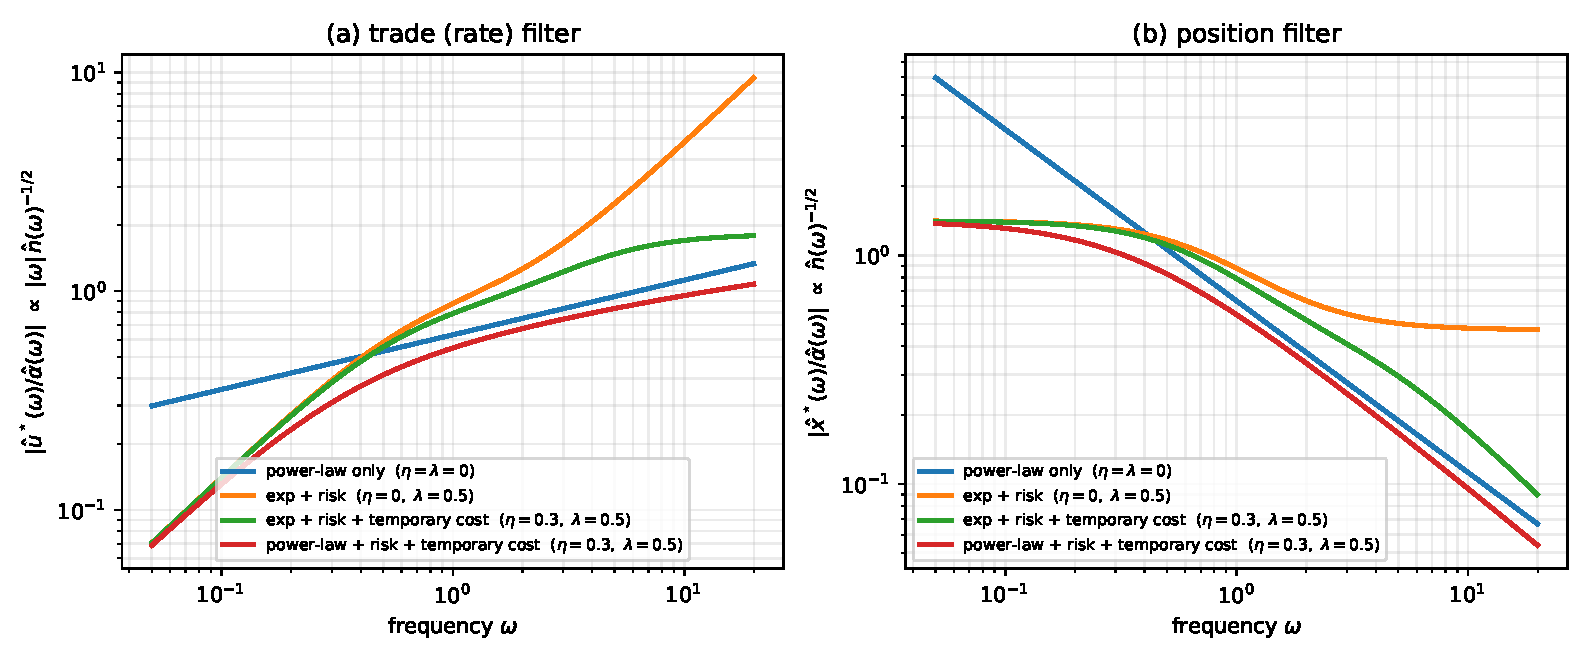
\includegraphics[width=\linewidth]{fig1_filter_magnitude}
\caption{The optimal filter per unit signal, across kernels ($\gamma=1$, $\kappa=2$, $\beta=0.5$). (a)~The trade (rate) filter $|\hat u^\star/\hat\alpha|\propto|\omega|\,\hat n(\omega)^{-1/2}$: without temporary cost the rate keeps growing at high frequency, the singular trading a short-memory kernel permits; temporary cost $\eta$ flattens it. (b)~The position filter $|\hat x^\star/\hat\alpha|\propto\hat n(\omega)^{-1/2}$ is low-pass, with the risk-aversion plateau, the exponential resilience shelf, and the fractional or temporary-cost rolloffs.}
\label{fig:filter}
\end{figure}

\subsection{Impact surfing}\label{sec:surfing}

Whether the optimal trade follows the signal or runs against it is a further difference between the kernels, decided by the response of the rate rather than the position. For an Ornstein--Uhlenbeck signal define the position response $X(\theta)=\E[x^\star_t\mid\alpha_t]/\alpha_t$ and the rate response $R(\theta)=\lim_{\epsilon\downarrow0}\E[u^\star_{t+\epsilon}\mid\alpha_t]/\alpha_t$; the latter is the average direction of the trade executed just after $t$ by a trader holding the current signal value. The forward limit handles the distribution-valued rate: for the exponential kernel with no temporary cost the optimal rate carries a contemporaneous white-noise atom correlated with $\alpha_t$, of weight
\begin{equation}\label{eq:c1}
c_1 \;=\; \lim_{|\omega|\to\infty}\frac{1}{\hat n_+(\omega)} \;=\; \frac{1}{\sqrt{2\gamma\kappa+\lambda}}\quad\text{(exponential)},\qquad c_1=0\quad\text{(power-law, or any $\eta>0$)};
\end{equation}
evaluating an instant later, where the intervening innovations are independent of $\alpha_t$, removes the atom and leaves the execution-relevant response.

\begin{proposition}[Rate response and the surfing threshold]\label{prop:response}
For rational or power-law symbols,
\begin{equation}\label{eq:response}
R(\theta) \;=\; \frac{\theta^2}{\Phi(\theta)}\Bigl[\frac{1}{\Phi(\theta)} - 2c_1\Bigr],
\end{equation}
with $c_1$ from \eqref{eq:c1}, while the position response $X(\theta)=\theta/\Phi(\theta)^2>0$ for every kernel. Positions never reverse; the rate reverses exactly when $2c_1\Phi(\theta)>1$. For the exponential propagator with no temporary cost, $\Phi=\sqrt A\,(m+\theta)/(\kappa+\theta)$ with $A=2\kappa\gamma+\lambda$ and $m=\kappa\sqrt{\lambda/A}$, and the rate reverses below the threshold
\begin{equation}\label{eq:threshold}
\theta^\ast \;=\; \kappa-2m \;=\; \kappa\Bigl[1-2\sqrt{\lambda/(2\kappa\gamma+\lambda)}\Bigr].
\end{equation}
For the power-law kernel, or any temporary cost, $c_1=0$ and $R(\theta)=\theta^2/\Phi(\theta)^2>0$ for every $\theta$.
\end{proposition}

The proof is in Appendix~\ref{app:C}. When the signal mean-reverts faster than the impact decays, $\theta>\kappa$ at $\lambda=0$, a signal-following trade would leave an impact residual that outlives the signal, and the optimal rate instead runs against the signal to ride that residual. Risk aversion lowers the threshold, and for $\lambda\ge2\kappa\gamma/3$ the optimal rate runs against the signal at every speed: the position stays aligned with the signal, but its mean reversion dominates the conditional rate. The pure-risk limit $R=-\theta^2/\lambda$ is the extreme case, a Markowitz position always conditionally exiting. For the power-law kernel the rate and position are aligned at every speed and risk aversion; the reversal does not occur there. Figure~\ref{fig:surf} shows the rate response and the resulting phase diagram.

\begin{figure}[t]
\centering
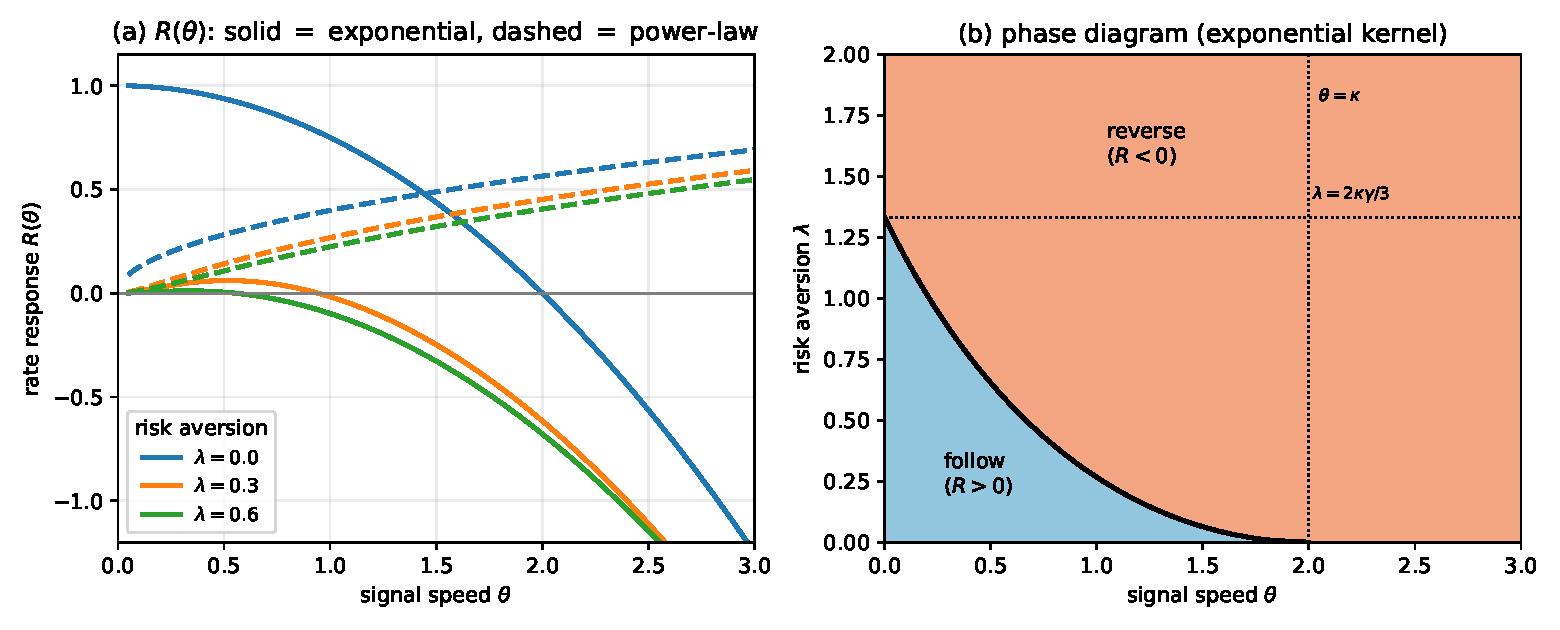
\includegraphics[width=\linewidth]{fig2_impact_surfing}
\caption{Direction of the optimal trade (exponential kernel, $\gamma=1$, $\kappa=2$). (a)~The rate response $R(\theta)$: the exponential kernel (solid) reverses sign at $\theta^\ast$, while the power-law kernel (dashed) stays positive at every risk aversion $\lambda$. (b)~Phase diagram: the optimum follows the signal ($R>0$) below the boundary $\theta^\ast(\lambda)$ and trades against it ($R<0$) above; the boundary meets the axes at $\theta=\kappa$ and $\lambda=2\kappa\gamma/3$.}
\label{fig:surf}
\end{figure}

This reversal profits from the trader's own residual impact, so it borders on the strategies that impact models are built to exclude. Positive-definiteness of the propagator, $\hat g\ge0$ in \eqref{eq:symbol}, rules out static round-trip arbitrage and, for the exponential and power-law kernels, transaction-triggered price manipulation \citep{Gatheral2010,AlfonsiSchiedSlynko2012}, so the reversal remains cost-optimal within the model class. It is the regime in which the optimum most exploits self-impact. The frictions omitted here --- bid--ask spread, position limits, order discreteness --- would temper it, and the prediction holds within the model where these are absent.

The vanishing atom is one face of a broader regularity: the power-law optimum never trades in blocks. A block trade --- a jump in the position --- pays a transient-impact cost proportional to the kernel at zero lag, $g(0)$, and for $g(t)=|t|^{-\beta}$ this is infinite. Instantaneous trading is therefore never optimal, neither on the whole line, where $c_1=0$ removes the lag-zero atom, nor at the ends of a finite horizon. A window with endpoints comes close: near a boundary the optimal rate diverges as $d(t)^{-\nu}$ in the distance $d(t)$ to the nearest endpoint (Proposition~\ref{prop:boundary}), the blow-up of the Gatheral--Schied--Slynko liquidation profile $[t(T-t)]^{-\nu}$ (Section~\ref{sec:powerlawFH}). The singularity is integrable ($\nu<\tfrac12$), so the position stays continuous and no discrete trade occurs. The exponential kernel is the opposite: $g(0)$ is finite, a block costs only finitely, and the optimal liquidation places discrete trades at both ends --- the block-plus-continuous strategy of \citet{ObizhaevaWang2013}, the finite-horizon counterpart of its white-noise atom.

These distinctions belong to the order-book resilience literature. \citet{AlfonsiSchiedSlynko2012} treat three questions together: whether an optimal execution trades in discrete blocks, whether it stays one-signed (their \emph{positive portfolio problem}), and whether the model admits price manipulation. The first two separate the kernels --- the power-law, with $g(0)=\infty$, trades in no blocks and, by the positive rate response \eqref{eq:response}, never reverses sign, while the exponential does both --- and the third is ruled out for either by the positive-definiteness $\hat g\ge0$ invoked above.

% =====================================================================
\section{The finite-horizon factorization}\label{sec:boundary}

The stationary theory of the previous sections describes an ongoing trading operation on the whole line. Most execution problems are posed instead on a fixed window $[0,T]$: a broker works a parent order over a session, or liquidates an inherited position by a deadline, ending flat, $x_T=0$. This is the optimal-execution problem, where the transient-impact literature began \citep{AlmgrenChriss2001,ObizhaevaWang2013,GatheralSchiedSlynko2012}. Two features are absent from the stationary theory: the two endpoints of the window, and the terminal inventory constraint. On $[0,T]$ translation invariance is lost, so the signal and friction no longer share a Fourier basis and the Szeg\H{o} formula does not apply.

The factorization survives the loss of translation invariance; only its computation changes. On the window the working variable is again the rate, which carries the terminal constraint and the endpoint blocks; the friction referred to the rate on $[0,T]$, $G_T=\eta I$ plus a continuous-kernel integral operator, is positive. Relative to the nest of adapted subspaces $\{P_{[0,t]}\}$ such an operator factors triangularly, $G_T=C_-C_+$ with $C_+$ a causal Volterra operator and $C_-=C_+^*$ \citep{GohbergKrein1970,Arveson1975}. Lemma~\ref{lem:pi} applies verbatim, and the optimum is
\begin{equation}\label{eq:finiteT}
u^\star \;=\; C_+^{-1}\,P_+\,C_-^{-1}\,\alpha^{\rm eff},
\qquad \alpha^{\rm eff} = \alpha + \sum_k \xi_k e_k,
\end{equation}
where $\alpha^{\rm eff}$ adjoins a multiplier $\xi_k$ for each linear position constraint $\langle e_k,x\rangle=0$, with a process-valued multiplier for the pathwise liquidation constraint $x_T=0$; each modifies the signal exactly as the adaptedness constraint does in \eqref{eq:multiplier}, confined to its constraint's annihilator, as in the constrained propagator problem of \citet{AbiJaberDeCarvalhoPham2024}. The Szeg\H{o} formula is replaced by a Volterra kernel, and nothing else in the construction moves.

\subsection{Relaxation to the stationary filter}\label{sec:bdrylayer}

The two endpoints and the terminal constraint act locally: their influence decays into the interior, where the finite-horizon policy relaxes to the stationary filter of \S\ref{sec:filter}. The bulk of a long session is governed by the whole-line solution, and only the start-up and terminal windows need separate treatment.

\begin{proposition}[Boundary-layer decay]\label{prop:boundary}
Let $u^{\star,T}$ be the finite-horizon optimum on $[0,T]$, $u^\star$ the whole-line stationary optimum for the same bounded signal, and $d(t)=\min(t,T-t)$ the distance to the nearest endpoint. Then, for constants $C(\beta)$, $C$ depending only on the kernel parameters,
\begin{equation}\label{eq:bdry-decay}
\bigl|u^{\star,T}_t - u^\star_t\bigr| \;\le\;
\begin{cases}
C(\beta)\,\|\alpha\|_\infty\,d(t)^{-\nu}, & \text{power-law kernel},\ \nu=\tfrac{1-\beta}{2},\\[3pt]
C\,\|\alpha\|_\infty\,e^{-b_1 d(t)}, & \text{rational symbol, } b_1 \text{ the slowest zero of } \hat n_+ .
\end{cases}
\end{equation}
\end{proposition}

The proof is in Appendix~\ref{app:D}. The boundary layer has width $\sim1/b_1$ for a rational kernel and is set by the impact memory for a power law; it is thin except for the small $\nu$ of the empirical power-law exponents, a quantitative statement of how long-memory impact makes horizons matter. Figure~\ref{fig:bdry} shows the finite-horizon rate tracking the stationary filter through the interior.

\begin{figure}[t]
\centering
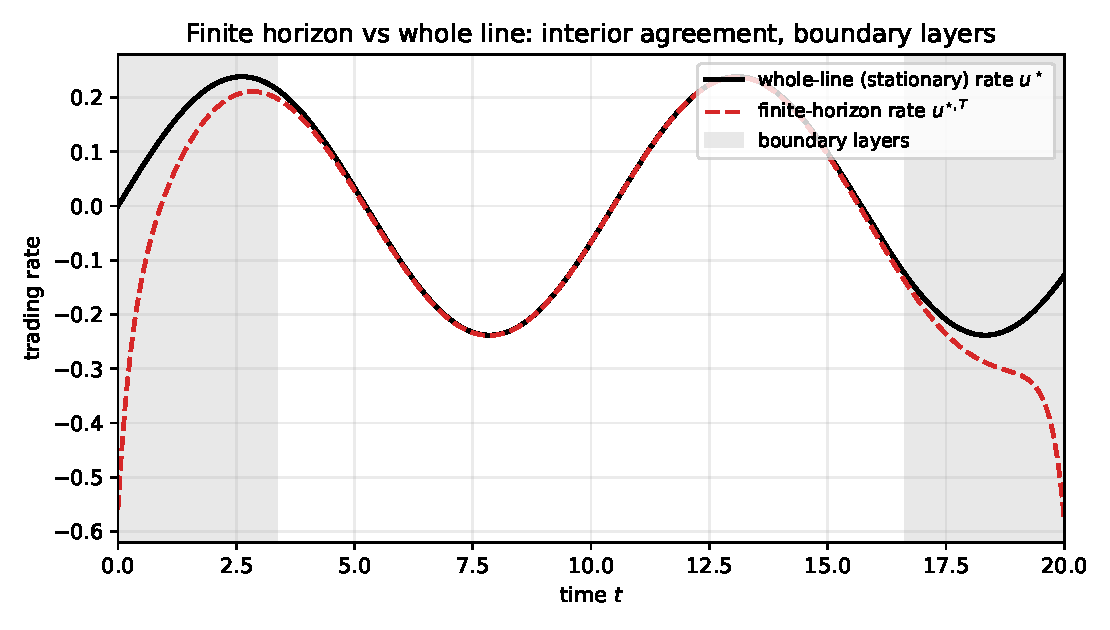
\includegraphics[width=0.72\linewidth]{fig3_boundary_layer}
\caption{Finite horizon versus whole line ($\eta=0.5$, $\gamma=1$, $\kappa=2$, $\lambda=1$, $T=20$). The finite-horizon optimal rate tracks the whole-line stationary rate through the interior and departs only in the start-up and terminal boundary layers, as quantified by Proposition~\ref{prop:boundary}; the shading marks the boundary-layer scale, not a fitted width.}
\label{fig:bdry}
\end{figure}

\subsection{The power-law factor}\label{sec:finiteT}

For a scale-free kernel the Volterra factor is explicit. For the power-law kernel ($\eta=\lambda=0$) the causal factor $C_+$ is the terminal-anchored Volterra operator with kernel
\begin{equation}\label{eq:gk-kernel}
c_+(t,s) = (\gamma c_\beta)^{1/2}\,\Bigl(\frac{T-s}{T-t}\Bigr)^{\!\nu}\frac{(t-s)^{\nu-1}}{\Gamma(\nu)},
\qquad 0\le s\le t\le T,
\end{equation}
verified by direct kernel integration, $C_-C_+=G_T$ including the constant. This is the whole-line fractional factor $I^\nu_+$ conjugated by multiplication by $(T-t)^\nu$: the terminal weight $((T-s)/(T-t))^\nu$ anchors the convolution factor to the endpoint $T$, and homogeneity of the kernel is what allows the anchoring to be a scalar weight. Each factor sees one endpoint, $C_+$ the terminal and its time reflection $C_-$ the initial; the identity \eqref{eq:pi} places the causal factor on the right of \eqref{eq:finiteT}, so the adapted projection sits between the factors and forces $C_+$ to anchor at $T$. Away from the endpoints the weight tends to one and $C_+$ tends to the whole-line factor, which is Proposition~\ref{prop:boundary} for this kernel.

\subsection{General kernels}\label{sec:gkgeneral}

Between the scale-free power law and the rational symbols of \S\ref{sec:rational} the factor is not explicit. The factorization $G_T=C_-C_+$ still exists \citep{GohbergKrein1970,Arveson1975}, but the factor kernel solves the Gohberg--Krein integral equations on $[0,T]$, with a closed form only in two classes: rational symbols, where it is a finite sum of endpoint-anchored exponential modes matched at the two boundaries, and scale-free kernels, where it is the conjugated fractional factor \eqref{eq:gk-kernel}. For a general propagator the equations are solved numerically.

% =====================================================================
\section{Recovery of earlier solutions}\label{sec:recovery}

The portfolio and execution rules of the literature are special cases of the factorization, in two groups. When the friction is stationary and rational --- pure risk, temporary cost, exponential resilience, and their combinations --- the Szeg\H{o} factor is a ratio of polynomials, and the optimal position is a finite sum of exponential moving averages of the signal (Section~\ref{sec:filter}); Markowitz, the G\^arleanu--Pedersen aim portfolio, and the stationary Neuman--Vo\ss{} solution are the cases with zero, one, and two averages. When the horizon is finite, the Gohberg--Krein factor of Section~\ref{sec:finiteT} takes over, producing the liquidation profiles of the execution literature --- the power-law U-shape and Fredholm solutions, and the exponential block-plus-continuous strategy of Obizhaeva--Wang. Beyond these two, a general propagator has no closed factor; \S\ref{sec:general} identifies the factorization with the general-propagator solutions of the literature.

\subsection{Stationary filters: rational frictions}\label{sec:rational}

For a rational symbol the optimal position is a finite sum of exponential moving averages of the return signal: their rates are the zeros of $\hat n_+$, their number is the number of poles, and risk aversion sets their scale. Each solution below is the outer factor of a particular rational symbol, read in the interior; the trade is the derivative of the position it prescribes.

\emph{Risk alone: the Markowitz rule.} With $\eta=\gamma=0$ the symbol is the constant $\hat n\equiv\lambda$, the factorization is trivial, and the \emph{position} is the memoryless mean--variance rule $x^\star_t=\mu_t/\lambda=\E_t[-\dot\alpha_t]/\lambda$ of \citet{Markowitz1952,Merton1971}, the expected return over risk aversion. The position responds to the return $\mu$, whereas under temporary impact alone (Section~\ref{sec:fractional}) the trading \emph{rate} is proportional to the appreciation signal $\alpha$. For an Ornstein--Uhlenbeck signal $\mu_t=\theta\alpha_t$, and the value is $v=\theta\sigma^2/4\lambda$.

\emph{Temporary cost with risk: the aim portfolio.} With $\gamma=0$ the friction is the differential operator $N=\lambda-\eta\,\partial_t^2$, local like the Markowitz case, and no factorization is needed. Conditioning the first-order condition \eqref{eq:foc} on $\F_t$ for $t\le s$, the planned path $m(s)=\E_t[x^\star_s]$ solves $Nm=\bar\mu(t,\cdot)$ driven by the forecast return, with $m(t)=x^\star_t$. Admissibility discards the growing mode $e^{as}$, $a=\sqrt{\lambda/\eta}$, and the executed rate is the initial slope of the plan, $u^\star_t=\dot m(t^+)$. Solving,
\begin{equation}\label{eq:gp}
u^\star_t = a\,(\mathrm{aim}_t - x^\star_t), \qquad
\mathrm{aim}_t = \frac{a}{\lambda}\int_0^\infty e^{-a\tau}\,\bar\mu(t,t+\tau)\,d\tau,
\end{equation}
partial adjustment at speed $a$ toward a target, the expected future Markowitz positions $\bar\mu/\lambda$ averaged at the adjustment rate; the realized past drops out of the target. For the Ornstein--Uhlenbeck signal $\bar\mu(t,t+\tau)=e^{-\theta\tau}\mu_t$, so $\mathrm{aim}_t=\frac{a}{a+\theta}\,\frac{\mu_t}{\lambda}$, the Markowitz position discounted by the persistence factor $a/(a+\theta)$. Integrating the adjustment, the position is one exponential moving average of the aim, hence of the signal, $x^\star_t=a\int_{-\infty}^t e^{-a(t-s)}\,\mathrm{aim}_s\,ds$. The general theory returns the same policy: the quadratic symbol factors by inspection, $\hat n=\eta\omega^2+\lambda=\bigl[\sqrt\eta\,(a-i\omega)\bigr]\bigl[\sqrt\eta\,(a+i\omega)\bigr]$, and \eqref{eq:ou-filter} with $\hat n_+=\sqrt\eta\,(a-i\omega)$ is the single-average filter just found. This is the continuous-time aim portfolio of \citet{GarleanuPedersen2016} (discrete time, \citet{GarleanuPedersen2013}; general targets, \citet{BankSonerVoss2017}): a diagonal friction gives exactly one pole.

\emph{Exponential propagator with risk.} For $g=e^{-\kappa|t|}$ and $\eta=0$,
\begin{equation}\label{eq:exp-factor}
\hat n_+ = \sqrt A\,\frac{m-i\omega}{\kappa-i\omega}, \qquad A=2\kappa\gamma+\lambda,\quad m=\kappa\sqrt{\lambda/A},
\end{equation}
and \eqref{eq:ou-filter} becomes the current signal plus one exponential moving average,
\begin{equation}\label{eq:ema}
x^\star_t \;=\; \frac{\kappa+\theta}{A(m+\theta)}\Bigl[\mu_t + (\kappa-m)\!\int_{-\infty}^t e^{-m(t-s)}\mu_s\,ds\Bigr],
\end{equation}
whose rate $m$ travels from $0$ to $\kappa$ as risk aversion grows. Exponential resilience with an Ornstein--Uhlenbeck signal is the model of \citet{LehalleNeuman2019}, whose explicit solution is the risk-free, singular finite-horizon liquidation generalizing \citet{ObizhaevaWang2013}; \eqref{eq:ema} is its stationary, no-temporary-cost form, risk aversion holding the position in place of the horizon.

\emph{Exponential propagator with temporary cost and risk.} The symbol is rational, and the outer factor
\begin{equation}\label{eq:nv-factor}
\hat n_+ = \sqrt\eta\,\frac{(b_1-i\omega)(b_2-i\omega)}{\kappa-i\omega}, \qquad
b_1^2b_2^2 = \frac{\lambda\kappa^2}{\eta}, \quad
b_1^2+b_2^2 = \kappa^2 + \frac{2\kappa\gamma+\lambda}{\eta},
\end{equation}
has two zeros $b_1,b_2$, so \eqref{eq:ou-filter} becomes a two-average filter,
\begin{equation}\label{eq:nv-filter}
x^\star_t \;=\; \frac{1}{\Phi(\theta)\sqrt\eta}\sum_{i=1}^2 w_i\!\int_{-\infty}^t e^{-b_i(t-s)}\mu_s\,ds,
\qquad w_i = \frac{\kappa-b_i}{b_j-b_i}.
\end{equation}
\citet{NeumanVoss2022} solve this by a system of coupled forward--backward SDEs and give the strategy as a feedback control; its gains reduce, in the stationary regime, to these two rates and two weights, the zeros and residues of the symbol, and the finite-horizon gains converge to them in the interior, the closed-loop poles equalling the moving-average rates $b_1,b_2$. Both degenerations are exact: at $\gamma=0$ the rates are $\{a,\kappa\}$ and the $\kappa$-pole cancels the kernel zero, recovering \eqref{eq:gp}; as $\eta\to0$, $b_1\to m$ and $\sqrt\eta\,(b_2-i\omega)\to\sqrt A$, recovering \eqref{eq:ema}. A rational friction with $n$ poles gives a filter with at most $n$ averages.

\subsection{Finite-horizon liquidation profiles}\label{sec:powerlawFH}

On a finite horizon the liquidation profiles of the execution literature follow from \eqref{eq:finiteT}. For a power-law kernel and a constant signal the projection is trivial and \eqref{eq:finiteT} reduces to $G_T^{-1}\mathbf 1$ up to the terminal-inventory multiplier, the U-shaped profile $u^\star(t)\propto[t(T-t)]^{(\beta-1)/2}$ of \citet[Ex.~2.30]{GatheralSchiedSlynko2012}. The exponential kernel gives the rational counterpart: a discrete block at each endpoint and continuous trading between, the block-plus-continuous liquidation of \citet{ObizhaevaWang2013}, its two blocks the finite-horizon form of the white-noise atom of \S\ref{sec:surfing} --- block trades replacing the integrable spike as $g(0)$ passes from infinite to finite. For a Gaussian Volterra signal, the first-order condition of the finite-horizon problem is the stochastic Fredholm equation that \citet{FordeSanchezSmith2022} solve on the Wiener chaos; the time reflection of \eqref{eq:gk-kernel} is the left-anchored outer factor they use to invert $G_T$ in full, where the factor order is immaterial. \eqref{eq:finiteT} is its solution operator, and expanding it on the chaos reproduces their Fredholm systems, with the generalized Abel inversion of \citet{ChakrabartiGeorge1994} implementing $G_T^{-1}$ and weighted Riemann--Liouville operators the individual factors.

\subsection{General propagators}\label{sec:general}

A general propagator has no closed factor (\S\ref{sec:gkgeneral}), so the explicit rules above do not apply, but the factorization still represents the solution. The adapted optimum of \eqref{eq:objective} is unique (Theorem~\ref{thm:general}), so the Gohberg--Krein policy \eqref{eq:finiteT} and the general-propagator solutions of the literature are one process written several ways: the free-boundary backward SDE and operator Riccati equation of \citet{AbiJaberNeuman2025}, the operator resolvents of \citet{AbiJaberNeumanTuschmann2024}, and the stochastic Fredholm equation with constraint multipliers of \citet{AbiJaberDeCarvalhoPham2024}. On $[0,T]$ the identification is term by term: the iterative solution of the stochastic Fredholm equation is the Neumann expansion that the Gohberg--Krein factors sum in closed form. In the stationary regime the Szeg\H{o} factor gives the closed-form filter of \S\ref{sec:filter}.

In the interior the finite-horizon solution relaxes to that stationary filter (Proposition~\ref{prop:boundary}, proved for the rational and power-law kernels and expected more generally). The rational filters of \S\ref{sec:rational} and the power-law profiles of \S\ref{sec:powerlawFH} are the two cases in which this interior solution is itself explicit.

% =====================================================================
\section{Concluding remarks}\label{sec:conclusion}

Trading against impact is a problem of timing. Unconstrained, the first-order condition is a single inversion of the friction operator; under adaptedness, with a friction that couples different times, the trader cannot truncate that inversion, because projection onto the past does not commute with the inverse. Factoring the friction along the filtration, into a causal part and its anticausal adjoint, resolves this, and the adapted inverse assembles from the one-sided factors. Sections~\ref{sec:fractional}--\ref{sec:recovery} apply that construction in different coordinates.

On the whole line the factor is a frequency-domain formula and the policy is a \emph{filter}, a transfer function that maps the observed signal to the position; the feedback solutions carry the same dependence in their state dynamics. Seen as an optimization, the policy is the projection of the unconstrained solution onto adapted strategies in the metric the friction sets, its Wiener--Hopf estimate from the past. The classical portfolio and execution rules are special cases: Markowitz when the friction is a constant, the aim portfolio when it is a second-order differential operator, and the moving-average filters of the resilience models.

The memory of the impact sets the shape of the policy. A rational kernel has finitely many relaxation rates, and the position is a finite sum of moving averages; a power-law kernel has a continuum, and the policy is a fractional derivative.

Three restrictions set the scope of these results. The costs are quadratic in the rate and position, so nonlinear impact lies outside the model. The explicit filters require a stationary Gaussian signal; for a general adapted signal, Theorem~\ref{thm:general} gives the policy through the forecast curve but not as a transfer function. And the asset is one-dimensional: a portfolio version calls for a matrix Wiener--Hopf factorization, which is explicit only in special cases.

% =====================================================================
\appendix

\section{Proof of Lemma~\ref{lem:pi} and Theorem~\ref{thm:general}}\label{app:A}
Causality of $A_+$ gives $(I-P_+)A_+P_+=0$, so $A_+$ and its causal inverse preserve the adapted subspace; taking adjoints and using $A_-=A_+^*$ gives $P_+A_-(I-P_+)=0$, so $A_-$ and $A_-^{-1}$ preserve the orthogonal complement. For adapted $v$, write $A_-v=P_+A_-v+(I-P_+)A_-v$; applying $A_-^{-1}$, the image of the second term stays in the complement and is annihilated by $P_+$, so $P_+A_-^{-1}P_+A_-v=P_+v=v$. Hence for adapted $u$,
\[
A_+^{-1}P_+A_-^{-1}\,(P_+AP_+)\,u = A_+^{-1}\bigl[P_+A_-^{-1}P_+A_-\bigr]A_+u = A_+^{-1}A_+u = u,
\]
using $P_+A_+u=A_+u$. The reverse composition equals the identity by the same bookkeeping, or from positivity of $P_+AP_+$ on the adapted subspace, for which a one-sided inverse is two-sided. For the pure power-law kernel the factors are unbounded and the computation holds on the dense domain of signals with $\int(1+\omega^2)S_\alpha(\omega)/\hat q(\omega)\,d\omega<\infty$ (Appendix~\ref{app:B}); any $\eta>0$ or $\lambda>0$ gives bounded inverses.

Theorem~\ref{thm:general} follows with $A=N$: strict convexity ($\hat n>0$ almost everywhere) makes \eqref{eq:foc} necessary and sufficient with a unique solution, which Lemma~\ref{lem:pi} inverts. The forecast-curve form follows from conditional Fubini: $N_-^{-1}$ has a deterministic anticausal kernel, so $\E_s[(N_-^{-1}\mu)(s)]$ integrates that kernel against $\E_s[\mu_r]=\bar\mu(s,r)$ for $r\ge s$. The rate form \eqref{eq:rate-policy} follows by differentiating \eqref{eq:policy}: $\partial_t\circ N_+^{-1}=Q_+^{-1}$, and on forecast curves $Q_-^{-1}=N_-^{-1}\circ(-\partial_s)$ with $-\partial_s\bar\alpha(s,\cdot)=\bar\mu(s,\cdot)$, so the whitened forecasts coincide, $\bigl(Q_-^{-1}\bar\alpha(s,\cdot)\bigr)(s)=\bigl(N_-^{-1}\bar\mu(s,\cdot)\bigr)(s)$.

\section{Proof of Theorem~\ref{thm:filter} and the Ornstein--Uhlenbeck formulas}\label{app:B}
The whitened return $N_-^{-1}\mu$ is the stationary filter of $\dot W$ with symbol $h=\hat\psi\,\hat n_-^{-1}$. Conditional expectation at $s$ annihilates innovations after $s$, so $P_+$ truncates the moving-average kernel at lag zero, acting as the plus-part $\pluspart{\,\cdot\,}$ on the symbol. Composing with $N_+^{-1}$ gives \eqref{eq:filter}; for $\lambda>0$ the symbol $\hat n$ is bounded below, so $h$ and the position filter lie in $L^2$. The hypothesis $\int(1+\omega^2)S_\mu(\omega)/\hat n(\omega)\,d\omega<\infty$ places $h$ in a Sobolev class on which the half-line indicator multiplies boundedly \citep[Ch.~1]{LionsMagenes1972}, giving $\hat\chi\in L^2$. For the value, the first-order condition and adaptedness give $v=\tfrac12\E[x^\star_t\mu_t]$, and by the It\^o isometry with $\overline{\hat\psi}=\hat n_+\overline h$ on the real axis, $\E[x^\star\mu]=\tfrac1{2\pi}\|\pluspart{h}\|^2$, which is \eqref{eq:value}.

Referred to the rate, the same argument with $A=Q$ gives $\hat\chi=\hat q_+^{-1}\pluspart{h_\alpha}$ and $v=\frac1{4\pi}\|\pluspart{h_\alpha}\|^2$ with $h_\alpha=\hat q_-^{-1}\hat\varphi$, valid whenever $h_\alpha\in L^2$, the power law at $\lambda=0$ included. The two forms agree where both apply: the moving-average symbols are related by $\hat\psi=\varphi(0)+i\omega\hat\varphi$, so $h-h_\alpha=\varphi(0)\,\hat n_-^{-1}$ is anticausal up to a lag-zero atom, and both parts are annihilated by the plus-part --- the atom because it loads on the contemporaneous innovation, which conditional expectation kills.

For the Ornstein--Uhlenbeck signal the collapse constant \eqref{eq:zeta-collapse} needs only the friction factor. With $\bar\mu(s,s+\tau)=\mu_s e^{-\theta\tau}$ and $f(\tau)=e^{-\theta\tau}$, closing the contour in the lower half-plane on the pole at $\omega=-i\theta$ gives $\rho=(N_-^{-1}f)(0)=\frac{1}{2\pi}\int\hat n_-(\omega)^{-1}(\theta-i\omega)^{-1}\,d\omega=1/\hat n_-(-i\theta)$, and $\hat n_-(-i\theta)=\hat n_+(i\theta)=\Phi(\theta)$ by conjugate symmetry. The stationary filter and value use the plus-part instead: $\hat\psi=\sigma\theta/(\theta-i\omega)$ and $h=\hat\psi\,\hat n_-^{-1}$. The combination
\[
h - \frac{\hat\psi}{\Phi(\theta)} = \sigma\theta\Bigl[\frac{1}{\hat n_-(\omega)} - \frac{1}{\hat n_-(-i\theta)}\Bigr]\frac{1}{\theta-i\omega}
\]
is anticausal: the bracket's pole at $\omega=-i\theta$ cancels, $\hat n_-^{-1}$ is analytic in the lower half-plane, and the product decays at infinity, carrying no atom. Hence $\pluspart{h}=\hat\psi/\Phi$, giving \eqref{eq:ou-filter} and, with $\|\hat\psi\|^2=\pi\sigma^2\theta$, the value $v=\sigma^2\theta/4\Phi^2$.

\section{Proof of Proposition~\ref{prop:response}}\label{app:C}
Write $\hat\varphi=\sigma/(\theta-i\omega)$ for the outer factor of $\alpha=\mu/\theta$, so the position filter is $\hat n_+^{-1}\hat\psi/\Phi=(\theta/\Phi)\hat n_+^{-1}\hat\varphi$. It vanishes at high frequency for every kernel considered, so $X(\theta)$ is the Laplace evaluation $\theta/\Phi(\theta)^2>0$. The rate filter $\hat\chi=(-i\omega)(\theta/\Phi)\hat n_+^{-1}\hat\varphi$ tends to $a_0=\theta\sigma c_1/\Phi$; splitting $\chi=a_0\delta+\chi_{\rm reg}$, the atom is excluded from the forward limit, and dominated convergence gives $R=(2\theta/\sigma^2)\sigma[\hat\chi(i\theta)-a_0]=\theta^2\Phi^{-1}[\Phi^{-1}-2c_1]$. For the exponential kernel with $\eta=0$, $\hat g(\omega)\omega^2\to2\kappa$, so $\hat n(\infty)=\lambda+2\gamma\kappa=c_1^{-2}$; the power-law kernel and any $\eta>0$ make $\hat n_+$ grow, so $c_1=0$. The threshold \eqref{eq:threshold} follows from $\Phi=\sqrt A(m+\theta)/(\kappa+\theta)$; consistency checks: $\lambda\to0$ on the exponential returns $R=(\kappa^2-\theta^2)/2\kappa\gamma$, and $\gamma\to0$ returns $R=-\theta^2/\lambda$.

\section{Proof of Proposition~\ref{prop:boundary}}\label{app:D}
The finite-horizon policy \eqref{eq:finiteT} differs from the stationary one through the terminal-anchored weight and the truncation of the factor kernels to $[0,T]$. For the power-law factor \eqref{eq:gk-kernel} the truncation cuts the Marchaud tail at distance $d(t)$, contributing $d(t)^{-\nu}$; the weight deviation $((T-s)/(T-t))^\nu=1+O(d(t)^{-1})$ is subdominant. For a rational symbol the causal factor $\hat n_+^{-1}$ has kernel decaying as $e^{-b_1\tau}$ at the slowest zero $b_1$ of $\hat n_+$, so truncation at distance $d(t)$ costs $e^{-b_1 d(t)}$; equivalently the finite-horizon feedback gains relax to their stationary values at rate $2b_1$.

\paragraph{Acknowledgements.} The author thanks CFM colleagues, and in particular Jean-Yves Audibert, Antoine Bambade, Raphael Benichou, Jean-Philippe Bouchaud, Raphael Maillet, Iacopo Mastromatteo and Marc Potters, for useful discussions. Research and write-up were assisted by Claude via the Feynman harness. 

\bibliographystyle{plainnat}
\bibliography{optimal-trading-filters}

\end{document}
